\chapter{Continuous Random Variables}

\section{Probability density functions}

A continuous r.v.\ takes values in an interval, such as a lifetime or a measurement error.
Since there are uncountably many values, individual values cannot carry positive
probability; instead probability is spread out according to a density.

\begin{definition}[Continuous r.v., p.d.f.]
A r.v.\ $X$ is \emph{continuous} if there is a function $f(x)\ge0$, the
\emph{probability density function} (p.d.f.), such that for all $a\le b$,
\[
  P(a \le X \le b) = \int_a^b f(x)\,dx, \qquad\text{with}\qquad \int_{-\infty}^\infty
  f(x)\,dx = 1.
\]
\end{definition}

\begin{theorem}[Basic facts]
\begin{enumerate}
  \item $P(X = a) = \int_a^a f(x)\,dx = 0$ for every $a$, so
        $P(a<X<b) = P(a\le X\le b)$: strict and non-strict inequalities agree.
  \item The c.d.f.\ $F(x) = P(X\le x) = \int_{-\infty}^x f(t)\,dt$ is continuous, and
        $f(x) = F'(x)$ wherever the derivative exists.
  \item $P(a < X \le b) = F(b) - F(a)$.
\end{enumerate}
\end{theorem}

\begin{important}[A density is not a probability]
$f(x)$ can exceed $1$. The meaningful statement is
$P(x < X \le x + \Delta x) \approx f(x)\Delta x$ for small $\Delta x$: $f(x)$ is
probability per unit length.
\end{important}

\begin{definition}[Mean and variance]
For continuous $X$,
\[
  \E[g(X)] = \int_{-\infty}^\infty g(x)f(x)\,dx, \qquad \mu = \E(X), \qquad
  \Var(X) = \E[(X-\mu)^2] = \E(X^2) - \mu^2.
\]
\end{definition}

All the properties of Chapter 6 (linearity, $\Var(aX+b) = a^2\Var(X)$, Chebyshev) carry
over, with sums replaced by integrals.

\begin{definition}[Quantiles]
For $0<p<1$, the $p$th \emph{quantile} (or $100p$th percentile) of $X$ is the value $q(p)$
with $F(q(p)) = p$. The \emph{median} is $q(0.5)$.
\end{definition}

\begin{example}[A worked density]
Let $f(x) = kx^2$ for $0 < x < 2$ and $0$ otherwise.
\begin{itemize}
  \item \emph{Constant:} $1 = \int_0^2 kx^2\,dx = 8k/3$, so $k = 3/8$.
  \item \emph{c.d.f.:} $F(x) = \int_0^x \frac38 t^2\,dt = x^3/8$ for $0\le x\le 2$, with
        $F(x) = 0$ for $x<0$ and $1$ for $x > 2$.
  \item \emph{A probability:} $P(X > 1) = 1 - F(1) = 1 - 1/8 = 7/8$.
  \item \emph{Median:} $m^3/8 = 1/2$ gives $m = 4^{1/3} \approx 1.587$.
  \item \emph{Mean:} $\E(X) = \int_0^2 \frac38 x^3\,dx = \frac38\cdot 4 = 1.5$.
  \item \emph{Variance:} $\E(X^2) = \int_0^2\frac38x^4\,dx = \frac38\cdot\frac{32}{5}
        = \frac{12}{5}$, so $\Var(X) = 2.4 - 2.25 = 0.15$.
\end{itemize}
\end{example}

\begin{center}
\begin{tikzpicture}
\begin{axis}[name=pdf, width=6.8cm, height=5cm, xmin=-0.3, xmax=2.5, ymin=0, ymax=1.7,
    xlabel={$x$}, ylabel={$f(x)$}, title={p.d.f.\ $\tfrac38x^2$}, title style={font=\small}, tick label style={font=\small}, label style={font=\small}, axis lines=left, scaled y ticks=false, yticklabel style={/pgf/number format/fixed}, samples=60]
  \addplot[draw=none, fill=blue!25, domain=1:2] {3*x^2/8} \closedcycle;
  \addplot[thick, blue!60!black, domain=0:2] {3*x^2/8};
  \draw[thick, blue!60!black] (axis cs:2,1.5) -- (axis cs:2,0);
  \draw[thick, blue!60!black] (axis cs:-0.3,0) -- (axis cs:0,0);
  \draw[thick, blue!60!black] (axis cs:2,0) -- (axis cs:2.5,0);
  \node[font=\small] at (axis cs:1.7,0.35) {$\tfrac78$};
  \node[font=\small, anchor=east] at (axis cs:1.3,1.2) {$P(X>1)$};
  \draw[->, gray] (axis cs:1.2,1.1) -- (axis cs:1.5,0.6);
\end{axis}
\begin{axis}[at={(pdf.east)}, anchor=west, xshift=1.2cm, width=6.8cm, height=5cm, xmin=-0.3,
    xmax=2.5, ymin=0, ymax=1.1, xlabel={$x$}, ylabel={$F(x)$}, title={c.d.f.\ $x^3/8$},
    title style={font=\small}, tick label style={font=\small}, label style={font=\small}, axis lines=left, scaled y ticks=false, yticklabel style={/pgf/number format/fixed}, samples=60]
  \addplot[thick, blue!60!black, domain=0:2] {x^3/8};
  \draw[thick, blue!60!black] (axis cs:-0.3,0) -- (axis cs:0,0);
  \draw[thick, blue!60!black] (axis cs:2,1) -- (axis cs:2.5,1);
  \draw[dashed, red!70!black] (axis cs:-0.3,0.5) -- (axis cs:1.587,0.5) -- (axis cs:1.587,0);
  \node[font=\small, anchor=south east] at (axis cs:1.55,0.52) {median $1.587$};
\end{axis}
\end{tikzpicture}
\end{center}

\section{Change of variables}

To find the distribution of $Y = h(X)$, the reliable method is to go through the c.d.f.

\begin{important}[The c.d.f.\ method]
\begin{enumerate}
  \item Write $F_Y(y) = P(Y \le y) = P(h(X)\le y)$ and rewrite this as an event about $X$.
  \item Express it using $F_X$.
  \item Differentiate: $f_Y(y) = F_Y'(y)$. Also find the range of $Y$.
\end{enumerate}
\end{important}

If $h$ is strictly increasing with inverse $h^{-1}$, this gives
$F_Y(y) = F_X(h^{-1}(y))$ and $f_Y(y) = f_X(h^{-1}(y))\,\frac{d}{dy}h^{-1}(y)$; for
decreasing $h$ there is a sign change, so in general
\[
  f_Y(y) = f_X(h^{-1}(y))\abs{\frac{d}{dy}h^{-1}(y)}.
\]

\begin{example}
With $X$ as in the previous example ($F_X(x) = x^3/8$ on $(0,2)$), let $Y = X^2$, which
takes values in $(0,4)$. For $0<y<4$,
\[
  F_Y(y) = P(X^2 \le y) = P(X\le\sqrt y) = \frac{y^{3/2}}{8}, \qquad
  f_Y(y) = \frac{3}{16}y^{1/2}.
\]
Check: $\int_0^4 \frac3{16}y^{1/2}\,dy = \frac{3}{16}\cdot\frac23\cdot 8 = 1$.
\end{example}

\section{Continuous uniform distribution}

\begin{definition}[Uniform]
$X\sim\Unif(a,b)$ if $f(x) = \dfrac{1}{b-a}$ for $a<x<b$ (and $0$ otherwise). Then
$F(x) = \dfrac{x-a}{b-a}$ for $a\le x\le b$.
\end{definition}

\begin{theorem}
If $X\sim\Unif(a,b)$, then $\E(X) = \dfrac{a+b}2$ and $\Var(X) = \dfrac{(b-a)^2}{12}$.
\end{theorem}

\begin{proof}
$\E(X) = \frac{1}{b-a}\int_a^b x\,dx = \frac{b^2-a^2}{2(b-a)} = \frac{a+b}{2}$, and
$\E(X^2) = \frac{b^3-a^3}{3(b-a)} = \frac{a^2+ab+b^2}{3}$. Subtracting $(a+b)^2/4$ gives
$(b-a)^2/12$.
\end{proof}

\begin{theorem}[Simulation by inverse c.d.f.]
If $F$ is a continuous, strictly increasing c.d.f.\ and $U\sim\Unif(0,1)$, then
$X = F^{-1}(U)$ has c.d.f.\ $F$.
\end{theorem}

\begin{proof}
$P(X\le x) = P(F^{-1}(U)\le x) = P(U\le F(x)) = F(x)$.
\end{proof}

This is how computers generate random numbers from other distributions starting from
uniform pseudo-random numbers.

\begin{center}
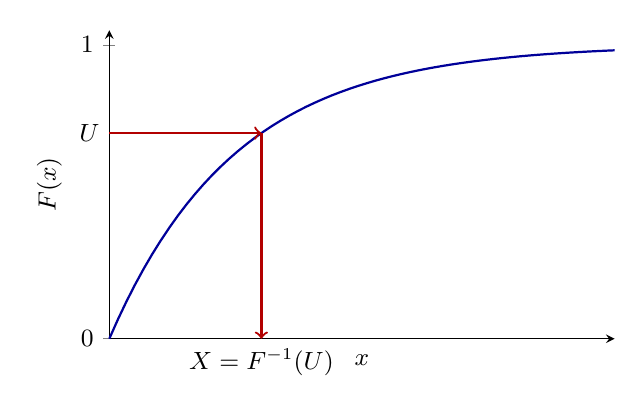
\begin{tikzpicture}
\begin{axis}[width=8cm, height=5.5cm, xmin=0, xmax=40, ymin=0, ymax=1.05, xlabel={$x$},
    ylabel={$F(x)$}, xtick=\empty, ytick={0,1}, clip=false, tick label style={font=\small}, label style={font=\small}, axis lines=left, scaled y ticks=false, yticklabel style={/pgf/number format/fixed}, samples=60]
  \addplot[thick, blue!60!black, domain=0:40] {1-exp(-x/10)};
  \draw[->, thick, red!70!black] (axis cs:0,0.7) -- (axis cs:12.04,0.7);
  \draw[->, thick, red!70!black] (axis cs:12.04,0.7) -- (axis cs:12.04,0);
  \node[anchor=east, font=\small] at (axis cs:0,0.7) {$U$};
  \node[anchor=north, font=\small] at (axis cs:12.04,0) {$X = F^{-1}(U)$};
\end{axis}
\end{tikzpicture}
\end{center}
Pick a uniform height $U$ on the vertical axis, run across to the c.d.f.\ and drop down:
regions where $F$ is steep (high density) catch many values of $U$.

\section{Exponential distribution}

\begin{definition}[Exponential]
$X\sim\Exp(\theta)$ (with $\theta>0$ the \emph{mean}) if
\[
  f(x) = \frac{1}{\theta}e^{-x/\theta}, \quad x>0; \qquad F(x) = 1 - e^{-x/\theta},
  \quad x\ge 0.
\]
Equivalently, with rate $\lambda = 1/\theta$, $f(x) = \lambda e^{-\lambda x}$.
\end{definition}

\begin{theorem}
If $X\sim\Exp(\theta)$, then $\E(X) = \theta$ and $\Var(X) = \theta^2$.
\end{theorem}

\begin{proof}
Substituting $y = x/\theta$ and using $\int_0^\infty y^n e^{-y}\,dy = n!$:
$\E(X) = \theta\int_0^\infty y e^{-y}\,dy = \theta$ and
$\E(X^2) = \theta^2\int_0^\infty y^2e^{-y}\,dy = 2\theta^2$, so
$\Var(X) = 2\theta^2 - \theta^2 = \theta^2$.
\end{proof}

\begin{theorem}[Waiting times in a Poisson process]
In a Poisson process with rate $\lambda$, the waiting time $X$ until the first event (from
any starting time) has an exponential distribution with mean $\theta = 1/\lambda$.
\end{theorem}

\begin{proof}
$X > x$ iff there are no events in $(0,x]$. The number of such events is $\Poi(\lambda x)$,
so $P(X > x) = e^{-\lambda x}$ and $F(x) = 1 - e^{-\lambda x}$.
\end{proof}

\begin{theorem}[Memoryless property]
If $X\sim\Exp(\theta)$, then for all $s,t\ge0$,
\[
  P(X > s + t \given X > s) = P(X > t).
\]
\end{theorem}

\begin{proof}
$\dfrac{P(X>s+t)}{P(X>s)} = \dfrac{e^{-(s+t)/\theta}}{e^{-s/\theta}} = e^{-t/\theta}$.
\end{proof}

An exponentially distributed lifetime does not ``age'': a component that has survived $s$
hours is as good as new. (The exponential is the only continuous distribution with this
property; the geometric is its discrete analogue.)

\begin{example}[Help desk again]
Calls arrive at rate $6$ per hour, i.e.\ $0.1$ per minute, so the waiting time $X$ (in
minutes) for the next call is $\Exp(\theta = 10)$.
\begin{itemize}
  \item $P(X > 15) = e^{-15/10} = e^{-1.5} \approx 0.2231$.
  \item Given no call in the first $10$ minutes, the probability of waiting more than
        $25$ minutes in total is $P(X>25\given X>10) = P(X > 15) \approx 0.2231$.
  \item Median: $1 - e^{-m/10} = 0.5$ gives $m = 10\ln 2 \approx 6.93$ minutes, less than
        the mean of $10$ because the distribution is right-skewed.
\end{itemize}
\end{example}

\begin{center}
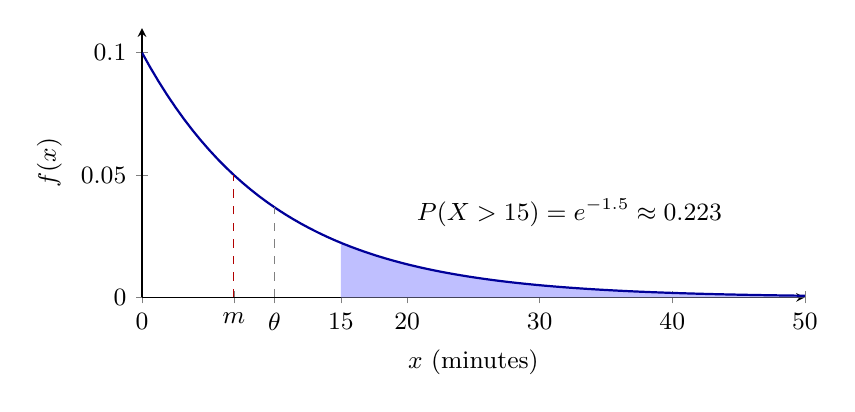
\begin{tikzpicture}
\begin{axis}[width=10cm, height=5cm, xmin=0, xmax=50, ymin=0, ymax=0.11, xlabel={$x$ (minutes)},
    ylabel={$f(x)$}, xtick={0,6.93,10,15,20,30,40,50}, xticklabels={0,$m$,$\theta$,15,20,30,40,50},
    tick label style={font=\small}, label style={font=\small}, axis lines=left, scaled y ticks=false, yticklabel style={/pgf/number format/fixed}, samples=80]
  \addplot[draw=none, fill=blue!25, domain=15:50] {exp(-x/10)/10} \closedcycle;
  \addplot[thick, blue!60!black, domain=0:50] {exp(-x/10)/10};
  \draw[dashed, red!70!black] (axis cs:6.93,0) -- (axis cs:6.93,0.05);
  \draw[dashed, gray] (axis cs:10,0) -- (axis cs:10,0.0368);
  \node[font=\small, anchor=south west] at (axis cs:20,0.025) {$P(X>15) = e^{-1.5}\approx 0.223$};
\end{axis}
\end{tikzpicture}
\end{center}
The $\Exp(10)$ density is highest at $0$ and has a long right tail, which pulls the mean
$\theta = 10$ above the median $m \approx 6.93$.

\subsection{The gamma function (brief)}

\begin{definition}[Gamma function]
For $\alpha > 0$, $\Gamma(\alpha) = \int_0^\infty y^{\alpha-1}e^{-y}\,dy$.
It satisfies $\Gamma(\alpha) = (\alpha-1)\Gamma(\alpha-1)$, $\Gamma(n) = (n-1)!$ for
positive integers $n$, and $\Gamma(1/2) = \sqrt\pi$.
\end{definition}

The gamma function makes integrals like $\int_0^\infty x^k e^{-x/\theta}dx =
\theta^{k+1}\Gamma(k+1)$ quick. The \emph{gamma distribution} (the waiting time to the
$k$th event of a Poisson process) and the \emph{chi-squared distribution} (the
distribution of $Z_1^2+\cdots+Z_k^2$ for independent standard normals) are built from it;
they are only mentioned in Stat 230 and are used properly in Stat 231.

\section{The normal distribution}

\begin{definition}[Normal]
$X\sim\Norm(\mu,\sigma^2)$ if
\[
  f(x) = \frac{1}{\sqrt{2\pi}\,\sigma}\exp\left(-\frac{(x-\mu)^2}{2\sigma^2}\right),
  \qquad -\infty<x<\infty.
\]
The \emph{standard normal} is $Z\sim\Norm(0,1)$, with p.d.f.\
$\varphi(z) = \frac{1}{\sqrt{2\pi}}e^{-z^2/2}$ and c.d.f.\ $\Phi(z)$.
\end{definition}

Note Stat 230 writes the second parameter as the \emph{variance}: $\Norm(100, 225)$ has
standard deviation $15$.

\begin{center}
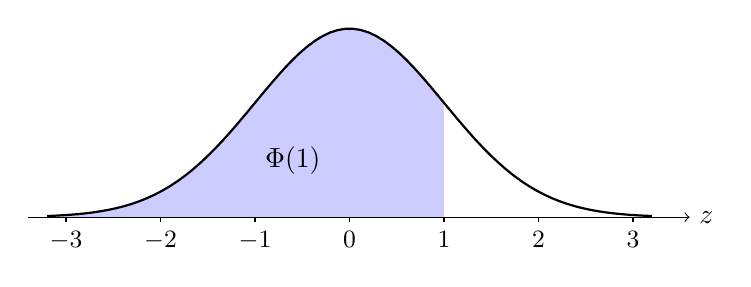
\begin{tikzpicture}[xscale=1.2, yscale=6]
  \fill[blue!20] (-3.2,0) -- plot[domain=-3.2:1,samples=60] (\x,{exp(-((\x)*(\x))/2)/sqrt(2*pi)}) -- (1,0) -- cycle;
  \draw[->] (-3.4,0) -- (3.6,0) node[right] {$z$};
  \draw[thick, domain=-3.2:3.2, samples=80] plot (\x,{exp(-((\x)*(\x))/2)/sqrt(2*pi)});
  \foreach \t in {-3,-2,-1,0,1,2,3} \draw (\t,0) -- (\t,-0.01) node[below] {\small $\t$};
  \node at (-0.6,0.12) {$\Phi(1)$};
\end{tikzpicture}
\end{center}

\begin{theorem}[Properties of the normal]
\begin{enumerate}
  \item $f$ is symmetric about $\mu$, bell-shaped, with inflection points at
        $\mu\pm\sigma$.
  \item $\E(X) = \mu$ and $\Var(X) = \sigma^2$.
  \item $\Phi(-z) = 1 - \Phi(z)$ (symmetry).
  \item (Standardising) If $X\sim\Norm(\mu,\sigma^2)$ then
        $Z = \dfrac{X-\mu}{\sigma}\sim\Norm(0,1)$, and more generally
        $aX+b\sim\Norm(a\mu+b, a^2\sigma^2)$.
\end{enumerate}
\end{theorem}

\begin{proof}[Proof of (4)]
$P(Z\le z) = P(X\le\mu+\sigma z) = \int_{-\infty}^{\mu+\sigma z} f(x)\,dx$. Substituting
$t = (x-\mu)/\sigma$ turns this into $\int_{-\infty}^z \varphi(t)\,dt$.
\end{proof}

The integral $\int\varphi$ has no closed form, so we use tables of $\Phi(z)$ (the
``N(0,1) table'' gives $\Phi(z)$ for $z = 0.00, 0.01, \dots, 3.49$) together with
symmetry. The table is reproduced in the last chapter.

\begin{important}[Using the N(0,1) table]
\begin{itemize}
  \item $P(Z\le z) = \Phi(z)$; \quad $P(Z > z) = 1 - \Phi(z)$.
  \item For negative $z$: $\Phi(-z) = 1 - \Phi(z)$.
  \item $P(a<Z<b) = \Phi(b) - \Phi(a)$; \quad $P(\abs Z < c) = 2\Phi(c) - 1$.
  \item Inverse lookup: find $z$ with $\Phi(z) = p$. Key values:
        $\Phi(1.2816) = 0.90$, $\Phi(1.6449) = 0.95$, $\Phi(1.96) = 0.975$,
        $\Phi(2.5758) = 0.995$.
\end{itemize}
\end{important}

\begin{example}[IQ scores]
Let $X\sim\Norm(100, 15^2)$.
\begin{itemize}
  \item $P(X > 120) = P\left(Z > \frac{120-100}{15}\right) = P(Z > 1.33) = 1 - 0.90824
        = 0.0918$ (using the table at $z = 1.33$; the exact value with $z=4/3$ is
        $0.0912$).
  \item $P(85 < X < 115) = P(-1 < Z < 1) = 2\Phi(1) - 1 = 2(0.84134) - 1 = 0.6827$.
  \item The 90th percentile: $\Phi(z) = 0.9$ at $z = 1.2816$, so
        $x = 100 + 1.2816(15) \approx 119.2$.
  \item $P(X < 80) = \Phi(-1.33) = 1 - 0.90824 = 0.0918$, by symmetry.
\end{itemize}
\end{example}

\begin{center}
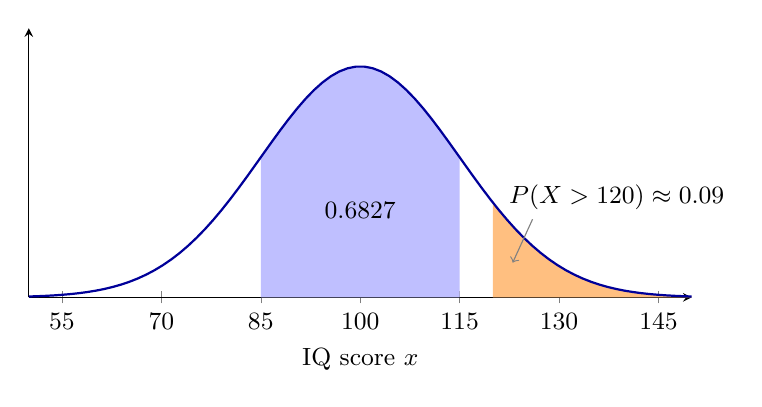
\begin{tikzpicture}
\begin{axis}[width=10cm, height=5cm, xmin=50, xmax=150, ymin=0, ymax=0.031, xlabel={IQ score $x$},
    xtick={55,70,85,100,115,130,145}, ytick=\empty, axis lines=left, tick label style={font=\small},
    label style={font=\small}, samples=80, clip=false]
  \addplot[draw=none, fill=blue!25, domain=85:115] {exp(-(x-100)^2/450)/(15*sqrt(2*pi))} \closedcycle;
  \addplot[draw=none, fill=orange!50, domain=120:150] {exp(-(x-100)^2/450)/(15*sqrt(2*pi))} \closedcycle;
  \addplot[thick, blue!60!black, domain=50:150] {exp(-(x-100)^2/450)/(15*sqrt(2*pi))};
  \node[font=\small] at (axis cs:100,0.01) {$0.6827$};
  \node[font=\small, anchor=south west] at (axis cs:121,0.009) {$P(X>120)\approx 0.09$};
  \draw[->, gray] (axis cs:126,0.009) -- (axis cs:123,0.004);
\end{axis}
\end{tikzpicture}
\end{center}

\begin{example}[Finding $\sigma$]
Bags of chips are filled with mean $\mu = 250$\,g. The machine's standard deviation is to
be set so that only $5\%$ of bags weigh less than $240$\,g. We need
$P(X<240) = \Phi\left(\frac{240-250}{\sigma}\right) = 0.05$, i.e.\
$-10/\sigma = -1.6449$, so $\sigma = 10/1.6449 \approx 6.08$\,g.
\end{example}

The ``68--95--99.7 rule'': for any normal distribution, about $68.3\%$, $95.4\%$ and
$99.7\%$ of the probability lies within $1$, $2$ and $3$ standard deviations of the mean.

\begin{center}
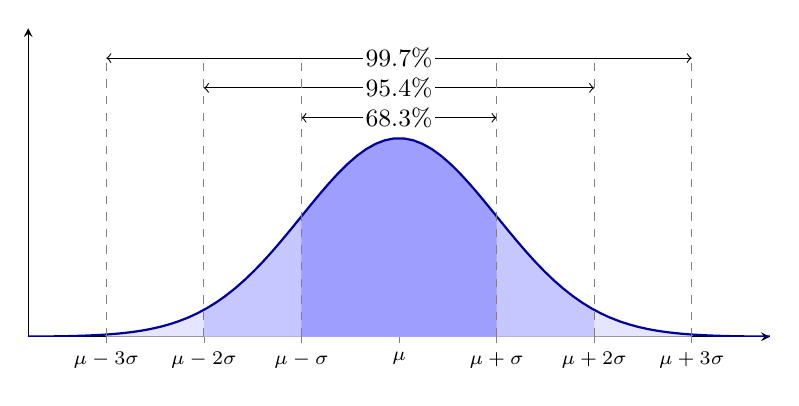
\begin{tikzpicture}
\begin{axis}[width=11cm, height=5.5cm, xmin=-3.8, xmax=3.8, ymin=0, ymax=0.62,
    xtick={-3,-2,-1,0,1,2,3}, xticklabels={$\mu-3\sigma$,$\mu-2\sigma$,$\mu-\sigma$,$\mu$,$\mu+\sigma$,$\mu+2\sigma$,$\mu+3\sigma$},
    ytick=\empty, axis lines=left, tick label style={font=\scriptsize}, samples=80]
  \addplot[draw=none, fill=blue!10, domain=-3:3] {exp(-x^2/2)/sqrt(2*pi)} \closedcycle;
  \addplot[draw=none, fill=blue!22, domain=-2:2] {exp(-x^2/2)/sqrt(2*pi)} \closedcycle;
  \addplot[draw=none, fill=blue!38, domain=-1:1] {exp(-x^2/2)/sqrt(2*pi)} \closedcycle;
  \addplot[thick, blue!60!black, domain=-3.8:3.8] {exp(-x^2/2)/sqrt(2*pi)};
  \draw[<->] (axis cs:-1,0.44) -- node[fill=white, font=\small, inner sep=1pt] {$68.3\%$} (axis cs:1,0.44);
  \draw[<->] (axis cs:-2,0.5) -- node[fill=white, font=\small, inner sep=1pt] {$95.4\%$} (axis cs:2,0.5);
  \draw[<->] (axis cs:-3,0.56) -- node[fill=white, font=\small, inner sep=1pt] {$99.7\%$} (axis cs:3,0.56);
  \draw[gray, dashed] (axis cs:-3,0) -- (axis cs:-3,0.56);
  \draw[gray, dashed] (axis cs:-2,0) -- (axis cs:-2,0.56);
  \draw[gray, dashed] (axis cs:-1,0) -- (axis cs:-1,0.56);
  \draw[gray, dashed] (axis cs:1,0) -- (axis cs:1,0.56);
  \draw[gray, dashed] (axis cs:2,0) -- (axis cs:2,0.56);
  \draw[gray, dashed] (axis cs:3,0) -- (axis cs:3,0.56);
\end{axis}
\end{tikzpicture}
\end{center}

\section{Summary}

\begin{itemize}
  \item A p.d.f.\ satisfies $f\ge0$, $\int f = 1$; probabilities are areas;
        $F' = f$; single points have probability zero.
  \item Distribution of $Y = h(X)$: work with $F_Y(y) = P(h(X)\le y)$ and differentiate.
  \item $\Unif(a,b)$: mean $(a+b)/2$, variance $(b-a)^2/12$.
  \item $\Exp(\theta)$: mean $\theta$, variance $\theta^2$, $P(X>x) = e^{-x/\theta}$,
        memoryless; waiting times in a Poisson process of rate $\lambda$ are
        $\Exp(1/\lambda)$.
  \item $\Norm(\mu,\sigma^2)$: standardise with $Z = (X-\mu)/\sigma$ and use the table of
        $\Phi$ with $\Phi(-z) = 1 - \Phi(z)$.
\end{itemize}
